\documentclass{article} % This command is used to set the type of document you are working on such as an article, book, or presenation

\usepackage{geometry} % This package allows the editing of the page layout
\usepackage{amsmath}  % This package allows the use of a large range of mathematical formula, commands, and symbols
\usepackage{graphicx}  % This package allows the importing of images
\usepackage{tikz} % This package allows the creation of graphics and diagrams
\usetikzlibrary{calc} % This library allows the use of advanced coordinate calculations

\newcommand{\maketitletwo}[2][]{\begin{center}
        \Large{\textbf{Assignment #1}
            
            Foundations of Audio Signal Processing} % Name of course here
        \vspace{5pt}
        
        \normalsize{Caspar Wiswesser, Vitezslav Kula, Prasun Dutta, Arash Astanboos % Your name here
        }
        \vspace{15pt}
        
\end{center}}
\begin{document}
    \maketitletwo[1]  % Optional argument is assignment number
    %Keep a blank space between maketitletwo and \question[1]
    
    \section*{Exercise 1.1}
    \subsection*{a)}
    \begin{equation*}
        (4-3i)(2+2i) = 8 + 8i - 6i + 6 = 14 + 2i
    \end{equation*}
    
    \subsection*{b)}
    \begin{equation*}
        (3-5i)^{-1} = \frac{1}{3-5i} = \frac{3+5i}{(3-5i)(3+5i)} = \frac{3+5i}{9+25} = \frac{3+5i}{34} = \frac{3}{34} + \frac{5}{34}i
    \end{equation*}

    \subsection*{c)}
    \begin{equation*}
        2e^{\frac{i\pi}{4}} + 2e^{i\pi} = 2 ( e^{\frac{i\pi}{4}} + e^{i\pi} ) = 2 ((-1)^{\frac{1}{4}} + (-1) = 2(-1)^{\frac{1}{4}} - 2 = \frac{2}{\sqrt{2}} + \frac{2i}{\sqrt{2}} - 2 = \sqrt{2} - 2 + \sqrt{2}i
    \end{equation*}

    \subsection*{d)}
    \begin{equation*}
        6i \left(\frac{1-i}{1+i}\right)^2 = 6i \left(\frac{(1-i)^2}{(1+i)^2}\right) = 6i \left(\frac{1-2i+i^2}{1+2i+i^2}\right) = 6i \left(\frac{1-2i-1}{1+2i-1}\right) = 6i \left(\frac{-2i}{2i}\right) = -6i
    \end{equation*}

    \subsection*{e)}
    \begin{align*}
        \frac{i(5-i)}{(1-i)(5+i)} &= \frac{5i+1}{5+i-5i-i^2} = \frac{5i+1}{6-4i} = \frac{(5i+1)(6+4i)}{(6-4i)(6+4i)} \\ 
        &= \frac{30i-20+6+4i}{36+24i-24i+16} = \frac{-14+34i}{52} = \frac{-7+17i}{26} \\
        &= -\frac{7}{26} + \frac{17}{26}i
    \end{align*}
        
    \section*{Exercise 1.2}
    
    \subsection*{a)}
    \begin{align*}
        1 + i \frac{1}{\sqrt{3}} \\
        z = a + bi \xrightarrow{} |z| = \sqrt{a^2 + b^2} : |z| = \sqrt{1 + \frac{1}{3}} = \sqrt{\frac{4}{3}} = \frac{2}{\sqrt{3}} \\
        |z| = \frac{2}{\sqrt{3}} = r : r (\cos{\phi} + i \sin{\phi}) = \frac{2}{\sqrt{3}} (\frac{\sqrt{3}}{2} + i \frac{1}{2}) \\
        \phi = \arctan{\left(\frac{\frac{1}{2}}{\frac{\sqrt{3}}{2}}\right)} = \arctan{\left(\frac{\sqrt{3}}{3}\right)} = \frac{\pi}{6} \\
        z = \frac{2}{\sqrt{3}} e^{i \frac{\pi}{6}}
    \end{align*}
    
    \begin{tikzpicture}[scale=2]
        % Draw polar coordinate system
        \draw[->] (-1.2,0) -- (1.2,0) node[right] {$\Re$};
        \draw[->] (0,-1.2) -- (0,1.2) node[above] {$\Im$};
        % Add values to the axis
        \foreach \x in {-1,-0.5,0.5,1} \draw (\x,0.1) -- (\x,-0.1) node[below] {$\x$};
        \foreach \y in {-1,-0.5,0.5,1} \draw (0.1,\y) -- (-0.1,\y) node[left] {$\y i$};
        % Plot point z
        \coordinate (z) at ({1}, {1/sqrt(3)});
        \fill (z) circle (1pt) node[above right] {$z$};
        \draw[dashed] (0,0) -- (z);
        \draw[->] (0.3,0) arc (0:30:0.3) node[midway,right] {$\phi$};
        \draw (0.8,0) arc (0:30:0.8) node[midway,right] {$r$};
    \end{tikzpicture}

    \subsection*{b)}
    \begin{align*}
        6 = a + bi \xrightarrow{} |z| = \sqrt{6^2 + 0} = 6 \\
        z = re^{i\phi} = 6 (\cos{\phi} + i \sin{\phi}) = 6 (1+0) \\
        \phi = \arctan{\left(\frac{0}{1}\right)} = 0 \\
        z = 6 e^{i0} = 6
    \end{align*}

    \begin{tikzpicture}[scale=2]
        % Draw polar coordinate system
        \draw[->] (-1.2,0) -- (6.2,0) node[right] {$\Re$};
        \draw[->] (0,-1.2) -- (0,1.2) node[above] {$\Im$};
        % Add values to the axis
        \foreach \x in {-1,1,2,3,4,5,6} \draw (\x,0.1) -- (\x,-0.1) node[below] {$\x$};
        \foreach \y in {-1,-0.5,0.5,1} \draw (0.1,\y) -- (-0.1,\y) node[left] {$\y i$};
        % Plot point z
        \coordinate (z) at ({6},0);
        \fill (z) circle (1pt) node[above right] {$z=6$};
        \draw[dashed] (0,0) -- (z);
    \end{tikzpicture}

    \subsection*{c)}
    \begin{align*}
        -4 + 4i = a + bi \xrightarrow{} |z| = |r| = \sqrt{(-4)^2 + 4^2} = 4 \sqrt{2} \\
        re^{i\phi} = r (\cos{\phi} + i \sin{\phi}) = 4 \sqrt{2} (-\frac{\sqrt{2}}{2} + i \frac{\sqrt{2}}{2}) \\
        \phi = \arctan{\left(\frac{\frac{\sqrt{2}}{2}}{-\frac{\sqrt{2}}{2}}\right)} = \frac{3\pi}{4} \\
        z = 4 \sqrt{2} e^{i \frac{3\pi}{4}}
    \end{align*}
    
    \begin{tikzpicture}[scale=1]
        % Draw polar coordinate system
        \draw[->] (-5,0) -- (1,0) node[right] {$\Re$};
        \draw[->] (0,-1.2) -- (0,5) node[above] {$\Im$};
        % Add values to the axis
        \foreach \x in {-4,-3,-2,-1,1} \draw (\x,0.1) -- (\x,-0.1) node[below] {$\x$};
        \foreach \y in {1,2,3,4} \draw (0.1,\y) -- (-0.1,\y) node[left] {$\y i$};
        % Plot point z
        \coordinate (z) at (-4,4);
        \fill (z) circle (1pt) node[above left] {$z$};
        \draw[dashed] (0,0) -- (z);
    \end{tikzpicture}

    \subsection*{d)}
    \begin{align*}
        (-1+i\sqrt{3})^4 = (a + bi)^4 = z^4 = (r e^{i\phi})^4 : r = \sqrt{1 + 3} = 2 \\
        2^4(-\frac{1}{2} + i \frac{\sqrt{3}}{2})^4 = 2^4 ((-\frac{1}{2})^2 - (\frac{\sqrt{3}}{2})^2 + i (-\frac{\sqrt{3}}{4} -\frac{\sqrt{3}}{4}))^2 = 2^4 (-\frac{1}{2} + i (-\frac{\sqrt{3}}{2}))^2 \\
        = 2^4 ((-\frac{1}{2})^2 - (-\frac{\sqrt{3}}{2})^2 + i (\frac{\sqrt{3}}{4} + \frac{\sqrt{3}}{4})) = 2^4 (-\frac{1}{2} + i \frac{\sqrt{3}}{2}) \\
        \phi = \arctan{\left(\frac{\frac{\sqrt{3}}{2}}{-\frac{1}{2}}\right)} = \frac{2\pi}{3} \\
        (z)^4=2^4(e^{i\frac{2\pi}{3}})
    \end{align*}

    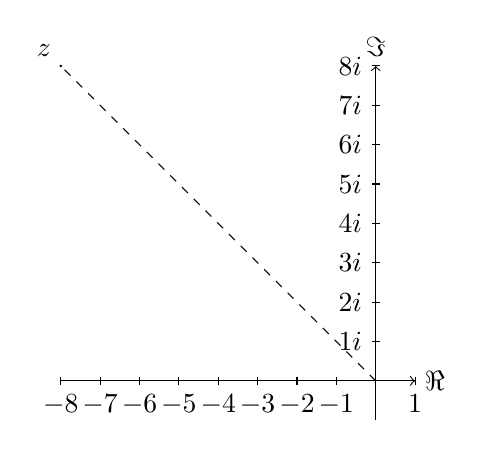
\begin{tikzpicture}[scale=0.5]
        % Draw polar coordinate system
        \draw[->] (-8,0) -- (1,0) node[right] {$\Re$};
        \draw[->] (0,-1) -- (0,8) node[above] {$\Im$};
        % Add values to the axis
        \foreach \x in {-8,-7,-6,-5,-4,-3,-2,-1,1} \draw (\x,0.1) -- (\x,-0.1) node[below] {$\x$};
        \foreach \y in {1,2,3,4,5,6,7,8} \draw (0.1,\y) -- (-0.1,\y) node[left] {$\y i$};
        % Plot point z
        \coordinate (z) at (-8,8);
        \fill (z) circle (1pt) node[above left] {$z$};
        \draw[dashed] (0,0) -- (z);
    \end{tikzpicture}


    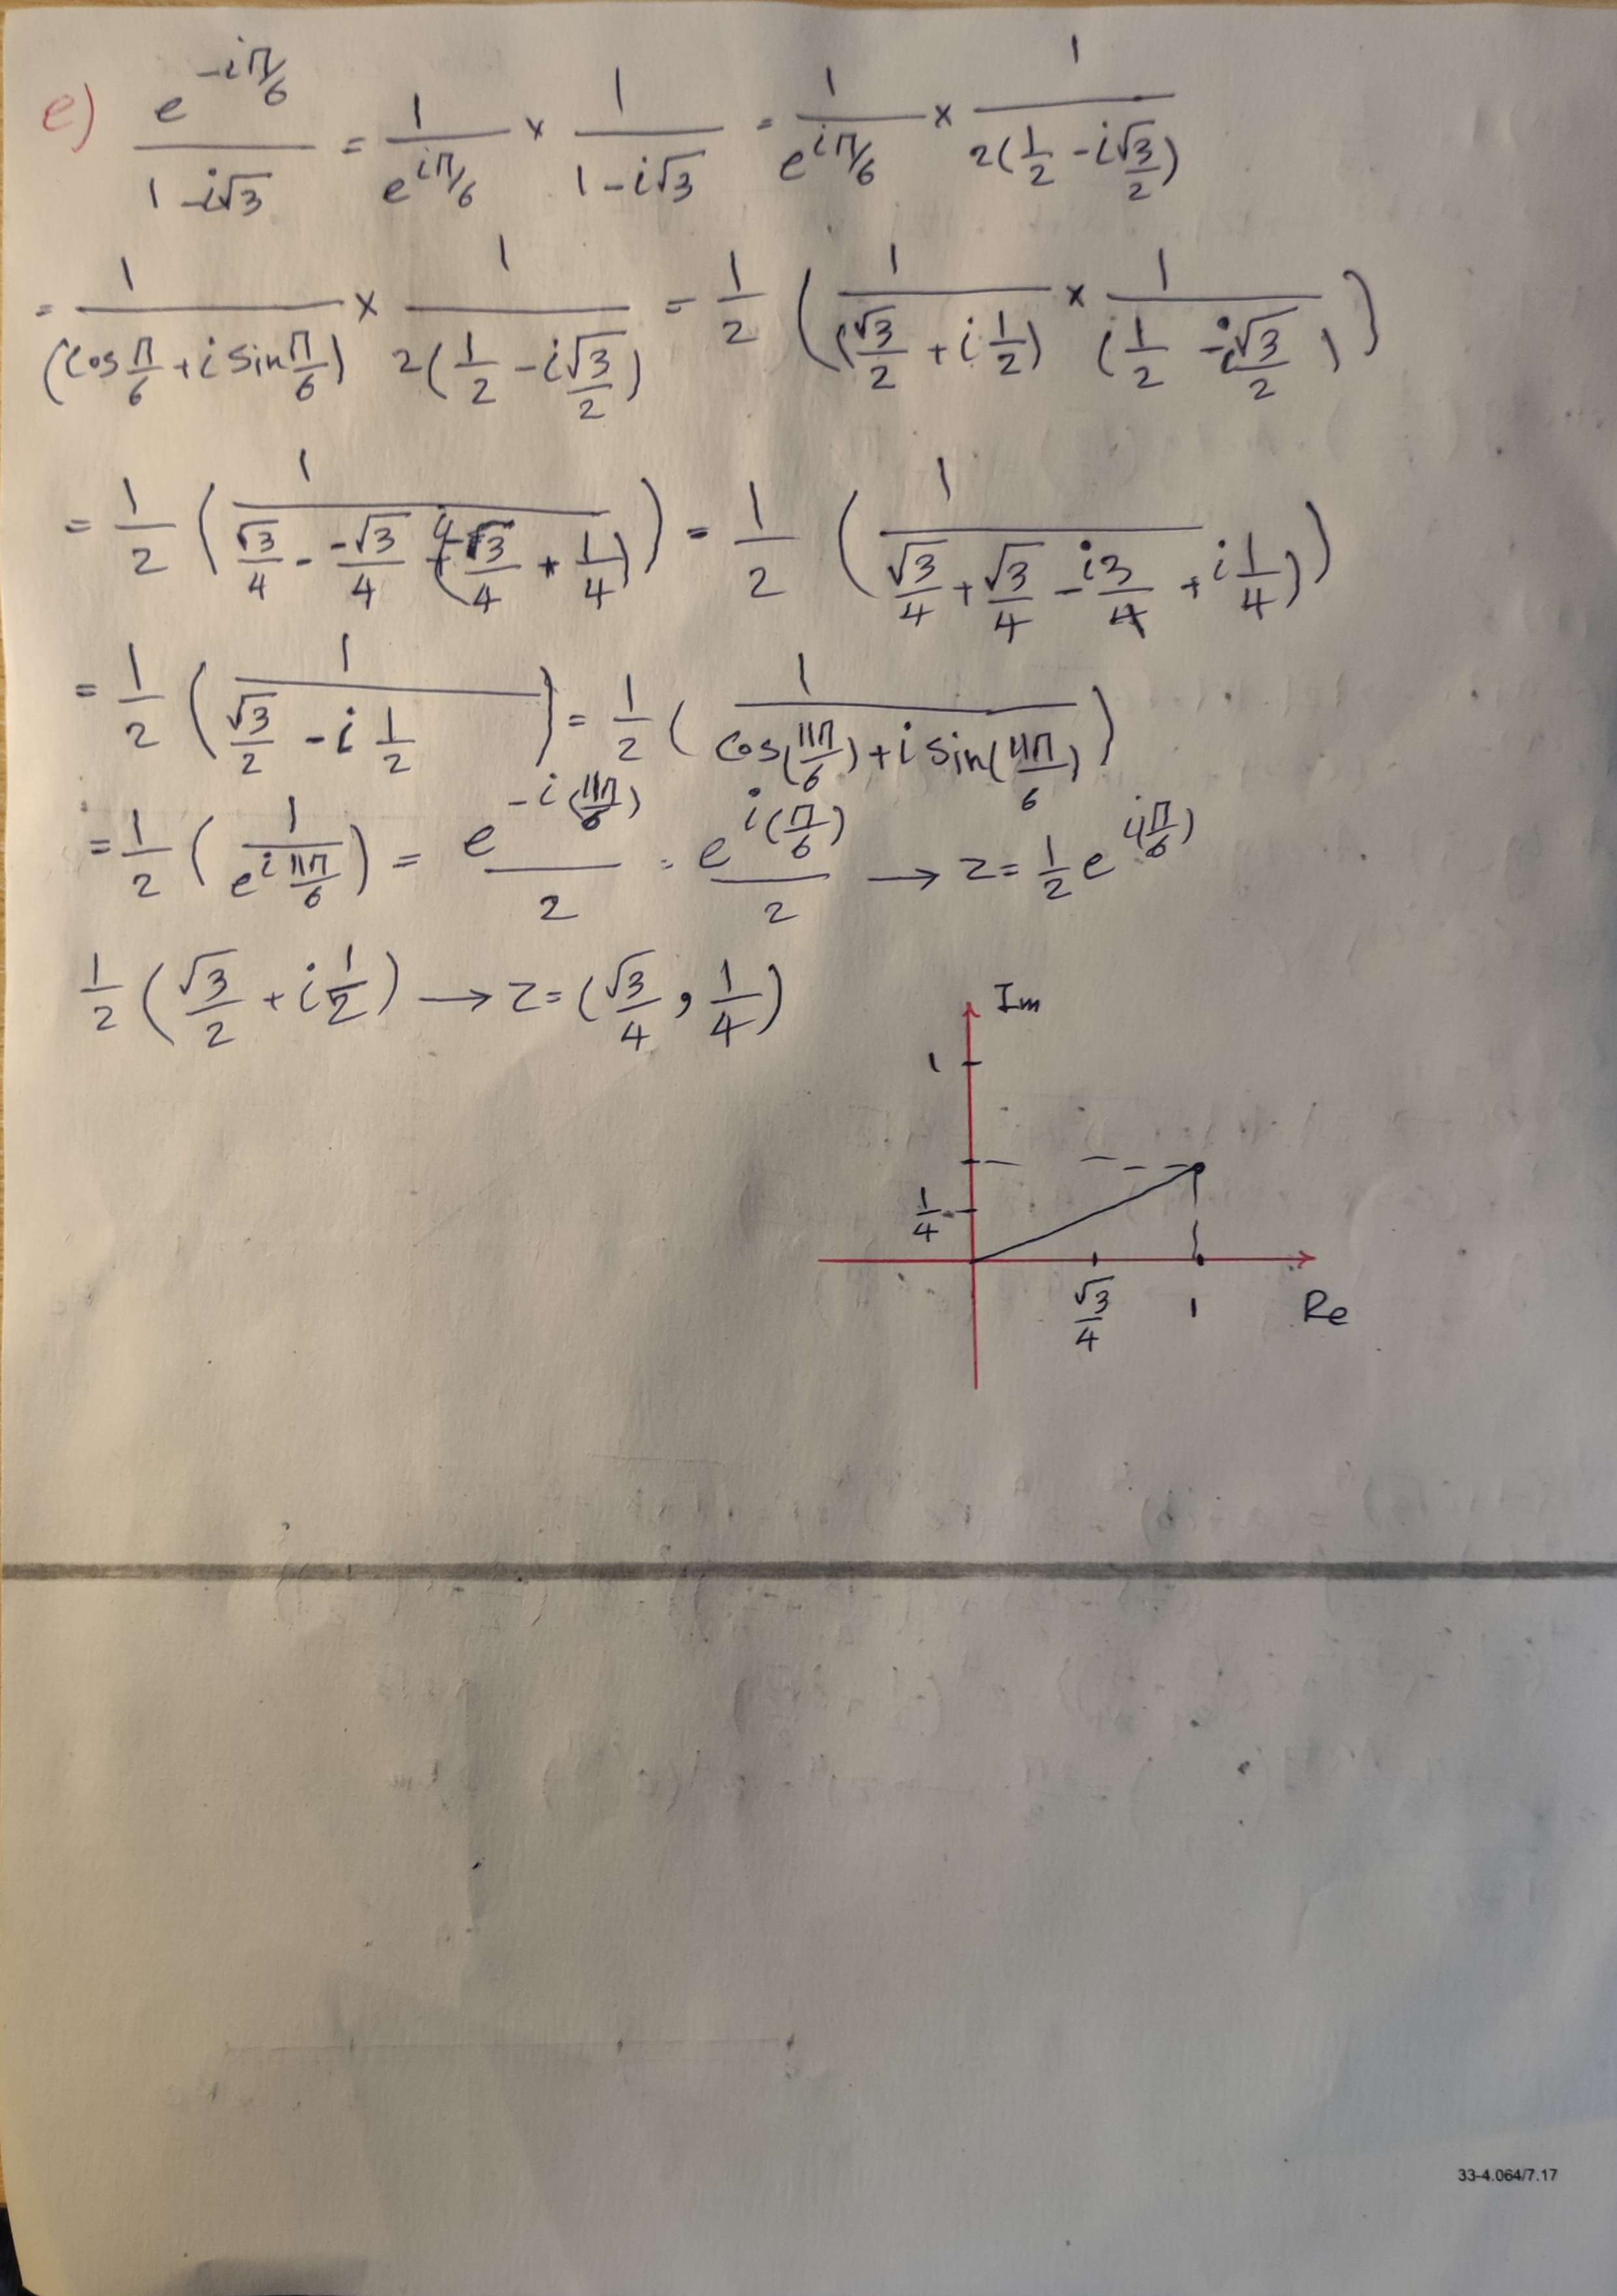
\includegraphics[width=\textwidth]{Exercise1.2e.jpg}
\end{document}-